\chapter{Introduction} 

This chapter introduces the interaction between CFS++ and a number of pre- and
postprocessing packages.

\section{Software Landscape}

\begin{figure}[htp]
  \begin{center}
    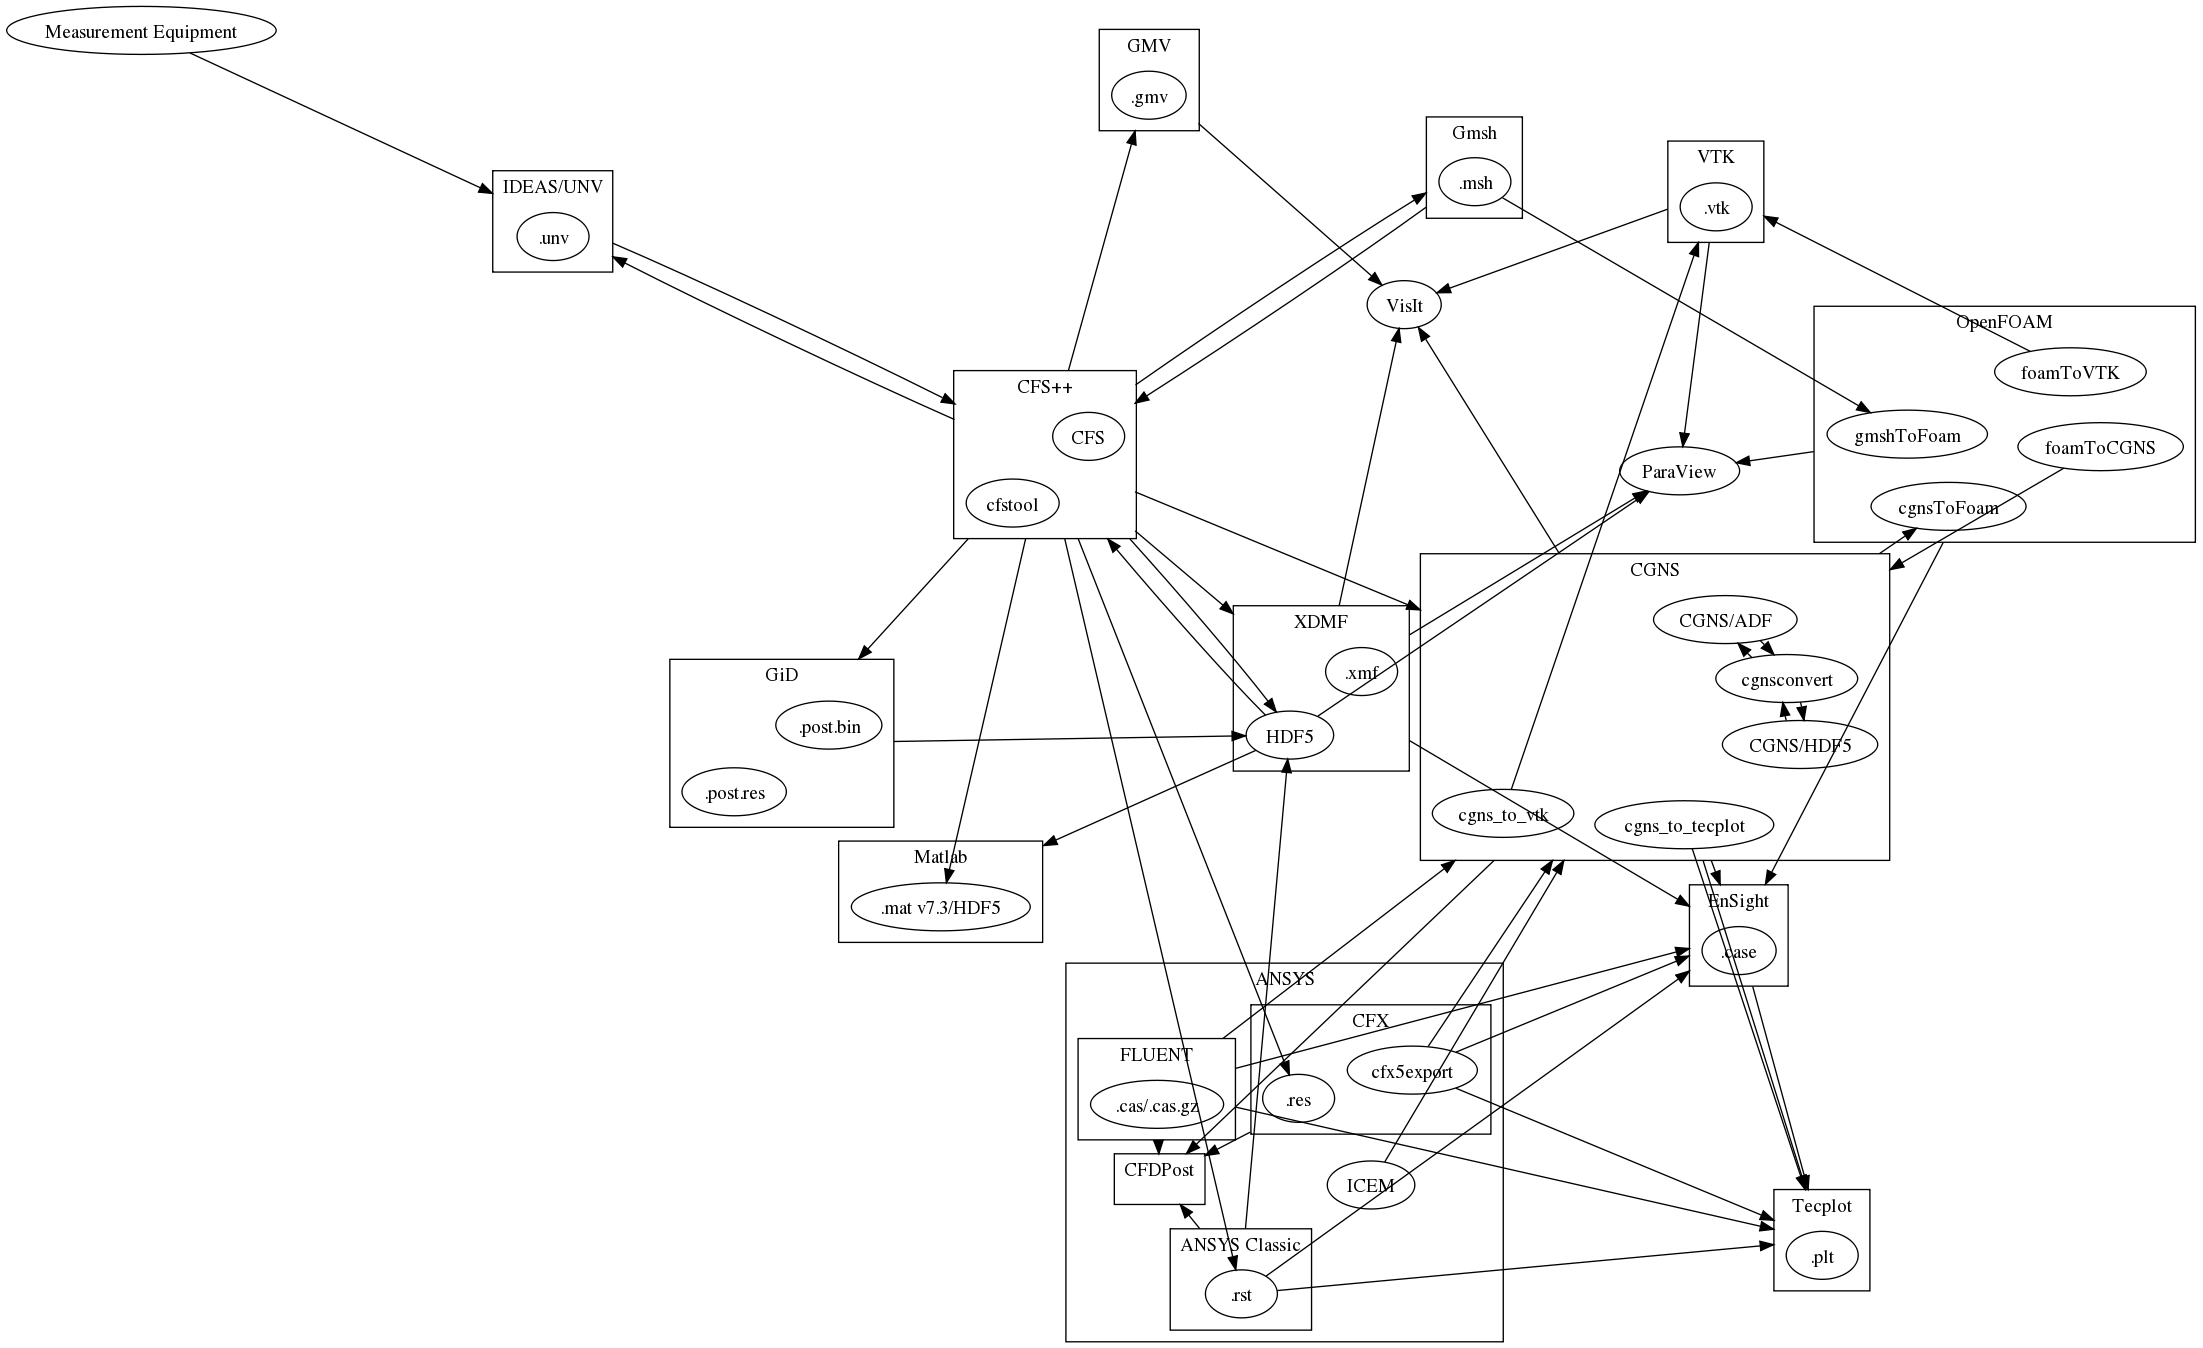
\includegraphics[width=\textwidth]{pics/soft_landscape} 
  \end{center}
  \caption{Software landscape for CFS++.}
  \label{fig:cfs_soft_landscape}
\end{figure}

\section{Pre- and Postprocessors}

\subsection{Mesh-based Tools}
\subsubsection{GiD} GiD  may be  downloaded along with  a free  one-month license
from    \url{http://gid.cimne.upc.es/download/official-versions}.    The   GiD
preprocessing    script    extension    for    CFS++   is    available    from
\url{https://lse17.e-technik.uni-erlangen.de:2001/svn/CAESAR.gid/trunk}. CFS++
can write the GiD postprocessing format, therefore data can be opened directly
in GiD.  Please  note, that the license servers  at Erlangen (131.188.140.136)
and  Klagenfurt  (rom,  143.205.120.86)  only provide  licenses  for  versions
9.x. In  order to register GiD,  start GiD, go to  Help $\rightarrow$ Register
GiD $\rightarrow$ select sysinfo for local host $\rightarrow$ enter IP address
of license server. For an introduction to modeling refer to the chapter 'Basic
Steps of Modeling in GiD' in \cite{Simkovics2010}.

\subsubsection{Gmsh}  If  you  have  installed  the  packages  provided  in  Sec.
\ref{sec:list_of_ext_packages} you should  already have Gmsh installed.  Since
CFS++ can  read the Gmsh  mesh format and  write into the  Gmsh postprocessing
format if USE\_GMSH is switched ON, no additional extensions are required. The 
official Gmsh download site is \url{http://geuz.org/gmsh/#Download}.

Please  refer  to  sections  \ref{sec:gmsh_pre}  and  \ref{sec:gmsh_post}  for
informations about pre- and postprocessing  of CFS++ meshes and results and to
Sec. \ref{sec:cfs_tool} for the possible ways of data conversion.


\subsubsection{ANSYS} An ANSYS Classic  APDL preprocessing extension is available
from  \url{https://lse17.e-technik.uni-erlangen.de:2001/svn/mkmesh/trunk}  for
generating  ASCII  based mesh  files  readable  by  CFS++.  An  extension  for
generating  HDF5 mesh files  based on  cplreader (cf.   Sec.  \ref{cplreader},
\cite{cplreadermanual} ) is  presented in Sec.  \ref{sec:ansys_mkmesh_mkhdf5}.
CFS++ can  write ANSYS  result files for  postprocessing if  the USE\_ANSYSRST
configuration option in CMake  is set to ON. This is the  case for the nightly
built executables ({\tt cfs\_nightly\_*, cfstool\_nightly\_*}) in Klagenfurt.

\textcolor{red}{ATTENTION:  The  ANSYS  Classic  GUI  requires  the  OpenMotif
library libXm.so.3.  Most modern Linux distributions, except openSUSE (package
name:  openmotif22-libs),  ship  with   LessTif.   On  Ubuntu  the  multiverse
repositories have  to be activated  in {\tt /etc/apt/sources.list}.   Then the
package  libmotif3  can be  installed.   Linking  the  libXm.so.2 provided  by
LessTif to libXm.so.3  does not work! In Klagenfurt we  solved this problem by
setting the library load path in our  own start scripts to a path containing a
valid libXm.so.3.}

For an introduction to modeling refer  to the chapter 'Basic Steps of Modeling
in   ANSYS'   in  \cite{Simkovics2010}.   Please   also   refer  to   sections
\ref{sec:ansys_pre} and  \ref{sec:ansys_post} for informations  about pre- and
postprocessing of CFS++ meshes and  results and to Sec. \ref{sec:cfs_tool} for
the possible ways of data conversion.


\subsubsection{ParaView} 
\url{http://daac.hpc.mil/paraview}

\url{http://www.paraview.org/paraview/help/documentation.html}

Tutorial auch Latex Sources
\url{http://www.vtk.org/Wiki/The_ParaView_Tutorial}

Tutorial for 3.10
\url{http://www.vtk.org/Wiki/images/2/2d/ParaViewTutorial310.pdf}

A ParaView plugin for reading CFS++'s native HDF5 format
is provided. It  will be built along ParaView,  if BUILD\_PARAVIEW is switched
ON in the CMake build environment of CFS++. Building ParaView will take a long
time, since also Qt4  must be built for it. Prebuilt binaries  for a number of
platforms  along  with  a few  sample  datasets  can  be  found on  the  CFS++
development                              server                             at
\url{https://lse17.e-technik.uni-erlangen.de:2001/files/precompiled/Paraview}. A
good   starting   point   for    the   ParaView   newbie   is   the   tutorial
\url{http://www.paraview.org/Wiki/images/8/88/ParaViewTutorial38.pdf}.   Please
refer to Sec. \ref{sec:paraview}  for further details about the implementation
of the CFS++ HDF5 plugin  and some advanced visualization techniques involving
data from CFS++.

CFS++  can  also  generate  Xdmf  \url{http://www.xdmf.org}  \cite{Clarke2002,
  Clarke2007} output which  can be read using ParaView.  When using Xdmf data,
also the  downloaded binaries from the  ParaView website may be  used since no
extra plugins are required any more.  This configuration will lack some of the
convenient  features  (e.g.  animation  of  harmonic results)  of  our  plugin
however.

\subsubsection{Installing SciPy/NumPy}
In  order  to be  able  to calculate  analytical  solutions  on meshes  inside
ParaView the SciPy and NumPy Python libs have to be present on the machine. An
installation          howto          can          be         found          at
\url{http://www.scipy.org/Installing_SciPy}.            The           pythonxy
\url{http://www.pythonxy.com}   distribution   may   also  be   a   noteworthy
alternative.

\subsubsection{VisIt}
VisIt    \url{https://wci.llnl.gov/codes/visit/}    is    another    VTK-based
visualization tool with broad support for CFD data formats. E.g. it has native
readers for  CGNS and  StarCCM+ files.  Like GMV it  is developed  at Lawrence
Livermore National Laboratories.  The main  data gateway from CFS++ is through
using Xdmf  files.  But  VisIt can also  read GMV  data files (at  least ASCII
ones).

\url{https://visualization.hpc.mil/wiki/VisIt}
\url{http://www.visitusers.org}
\url{https://wci.llnl.gov/codes/visit/doc.html}

\subsubsection{Tecplot}
Getting started Manual:
\url{http://download.tecplot.com/360/tpgs.pdf}

\url{http://www.tecplot.com/Training/GettingStarted.aspx}

\url{http://www.tecplot.com/Training/FeatureTutorials.aspx}

\url{http://www.genias-graphics.de/cms/tp-360-tutorials.html}

\subsubsection{EnSight}
EnSight \url{http://www.ensight.com} is a commercial postprocessor with support for a wide range of data formats. 
A nice short introduction to EnSight can be found at \url{http://www.scc.kit.edu/produkte/3847.php}. We also support reading EnSight data files with cplreader (cf. \cite{cplreadermanual}).

\url{http://daac.hpc.mil/ensight}

\url{http://www.ensight.com/Tutorials/}

EnSight 9 to 10: http://wiki.ensight.com/w/EnSight10Transition

\url{http://www.ensight10.com/sample-page/ensight-10-intro-tutorials/}

\subsubsection{ANSYS CFDPost}
CFD Post Users Guide:
\url{http://www1.ansys.com/customer/content/documentation/120/cfx/xpost.pdf}

\url{http://www1.ansys.com/customer/content/documentation/121/fluent/flcfd.pdf}
\url{http://www.cfd-online.com/Wiki/FLUENT}

\url{http://www.ansys.com/Products/Simulation+Technology/Fluid+Dynamics/ANSYS+CFD-Post}

\subsubsection{FieldView}

\subsubsection{Others}  The  GMV\footnote{\url{http://www.generalmeshviewer.com}}
postprocessor is  not publicly available any  more, but is  still installed at
Erlangen and Klagenfurt.   It may be obtained also  from the CFS++ development
server                                                                       at
\url{https://lse17.e-technik.uni-erlangen.de:2001/files/precompiled/GMV}. Also
refer  to Sec.   \ref{sec:gmv}  for  an introduction  on  using GMV.   Another
postprocessor, which  is capable  of reading  GMV files, is  free and  has its
roots      also     at      Lawrence     Livermore      Labs      is     VisIt
(\url{https://wci.llnl.gov/codes/visit/}).

The  hdfview  HDF5 viewer\footnote{\url{http://www.hdfgroup.org/hdf-java-html/hdfview}}
may be built  from source by switching the  BUILD\_HDFVIEW CMake configuration
option ON.

\subsection{Tools for In/Output Signal Processing}
\subsubsection{HDF5 Tools}
HDF5                                command                               line
tools\footnote{\url{http://www.hdfgroup.org/products/hdf5_tools/\#h5dist}} get
built along CFS++ in any case and are available in CFS\_BUILD\_DIR/bin/DISTRO.

\url{http://ab-initio.mit.edu/wiki/index.php/H5utils}

HDF5 in Perl:
\url{http://search.cpan.org/~cerney/PDL-IO-HDF5-0.63/}


\subsubsection{Matlab}
Matlab        can        also         read        and        write        HDF5
files\footnote{\url{http://www.mathworks.com/help/techdoc/ref/hdf5.html},
\url{http://www.scipy.org/Cookbook/hdf5_in_Matlab}}   and   is  available   in
Klagenfurt and Erlangen.

\subsubsection{Octave}

\begin{verbatim}
d = load('-hdf5', 'check.h5')
save -hdf5 out.mat
\end{verbatim}

Octave legt die Variablen in Groups ab und darin erst die Datensaetze:

\begin{verbatim}
octave:1> x = diag ([1,2,3]);
octave:2> x
x =

   1   0   0
   0   2   0
   0   0   3

octave:3> save -hdf5 foo.mat x
octave:4> system("h5ls foo.mat/x")
type                     Dataset {SCALAR}
value                    Dataset {3, 3}
ans = 0
octave:5> system("h5dump -d /x/value foo.mat")HDF5 "foo.mat" {DATASET "/x/value" {
   DATATYPE  H5T_IEEE_F64LE
   DATASPACE  SIMPLE { ( 3, 3 ) / ( 3, 3 ) }
   DATA {
   (0,0): 1, 0, 0,
   (1,0): 0, 2, 0,
   (2,0): 0, 0, 3
   }
}
}

ans = 0
\end{verbatim}

Dritte Spalte einlesen:

\begin{verbatim}
octave:14> system("h5dump -d /x/value -s 0,2 -S 1,1 -c 3,1 -k 1,1 foo.mat")
HDF5 "foo.mat" {
DATASET "/x/value" {
   DATATYPE  H5T_IEEE_F64LE
   DATASPACE  SIMPLE { ( 3, 3 ) / ( 3, 3 ) }
   SUBSET {
      START ( 0, 2 );
      STRIDE ( 1, 1 );
      COUNT ( 3, 1 );
      BLOCK ( 1, 1 );
      DATA {
      (0,2): 0,
      (1,2):  0,
      (2,2):  3
      }
   }
}
}
ans = 0
\end{verbatim}

\begin{verbatim}
octave:45> t=[0:100]
octave:47> t2 = t/100*2*pi
octave:48> sin = sin(t2)
octave:49> cos = cos(t2)
octave:51> matrix = [t2;sin;cos]
octave:52> save -hdf5 foo.mat matrix
octave:53> system("h5dump -d /matrix/value -y foo.mat | sed -n '/DATA {/,/}/p' | sed -e '1d' -e 's/,//g' -e '$d'")
\end{verbatim}


\subsubsection{Python Tools}

\cite{Langtangen2011, Langtangen2008, Alchin2010, Pilgrim2009, Pilgrim2004}

\url{http://www.pytables.org}

\url{http://alfven.org/wp/hdf5-for-python/}

\subsubsection{Gnuplot}


Gnuplot book: \cite{Janert2009} \url{http://fig.if.usp.br/~lucmod/tips/gnuplotbook.pdf}
Gnuplot website: \url{http://www.gnuplot.info/}

Plot HDF5 Data in GnuPlot:

\begin{verbatim}
plot "< magic_tool input file"
plot "< h5dump -d /matrix/value -y foo.mat | sed -n '/DATA {/,/}/p' | sed -e '1d' -e 's/,//g' -e '$d'" using 1:3
\end{verbatim}



